\documentclass{beamer} 
\usetheme{default} 
\setbeamercovered{transparent}

%\useoutertheme{umbcfootline} 
\setbeamertemplate{background canvas}[vertical shading][bottom=red!20,top=yellow!30] 


\usepackage[spanish]{babel}
%\usepackage[latin1]{inputenc}
\usepackage[utf8x]{inputenc}
\usepackage{multicol}


\title{Componentes GUI en Java}

\author{Manuel J. Molino Milla \and Luis Molina Garzón}

\date{\today} %

\institute{IES Virgen del Carmen \and Departamento de Informática}




%\beamerdefaultoverlayspecification{<+->}

\begin{document}


\begin{frame}
  \titlepage
\end{frame}

\begin{frame}
    \frametitle{Logo}
\begin{figure}

\includegraphics[scale=1]{imagenes/logo.jpeg} 
\caption{Logo Java}
\end{figure}
\end{frame}

\begin{frame}
  \frametitle{Contenido}
  \tableofcontents[pausesections]
\end{frame}



\section{Introduccion}


\begin{frame}
\frametitle{Introduccion}
\begin{itemize}[<+->]
\item Son las estructuras graficas que componen la interfaz de usuario.
\item Seran añadidas al contenendor de swing (generalmente un panel)
\item Generalmente se le asociara un evento para la interaccion con el usuario
\end{itemize}
\pause
\begin{center}
{\color{blue} \href{http://web.mit.edu/6.005/www/sp14/psets/ps4/java-6-tutorial/components.html}{Guia de componentes}}
\end{center}
\end{frame}

\section{Paneles}
\begin{frame}
\frametitle{Componentes}
\framesubtitle{Paneles intermedios}
\begin{figure}
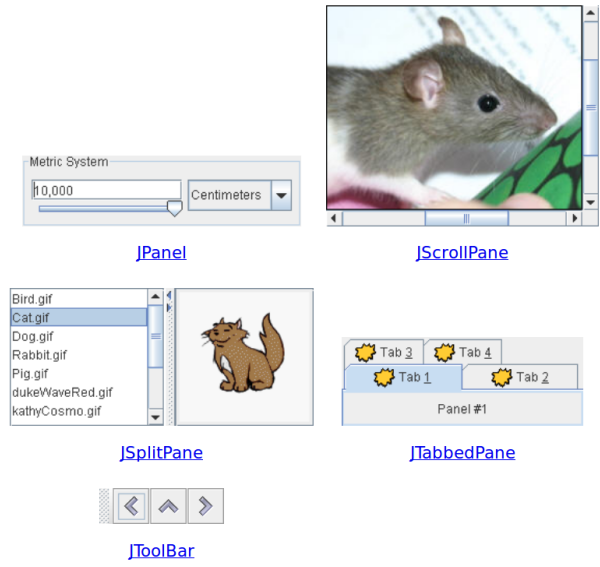
\includegraphics[scale=0.4]{imagenes/paneles.png}
\caption{Paneles}
\end{figure}
\end{frame}

\subsection{JPanel}


\begin{frame}[fragile]
\frametitle{JPanel}
\begin{itemize}[<+->]
\item Es un contenedor ligero.
\item Usado para agrupar componentes.
\item Tiene \emph{FlowLayout} como layout por defecto.
\item Ejemplo de uso;
\end{itemize}
\pause
\begin{verbatim}
JLabel label = new JLabel("Enter username:");
JTextField userName = new JTextField(20);
newPanel.add(label);
newPanel.add(userName);
\end{verbatim}
\end{frame}


\subsection{JScrollPane}
\begin{frame}
\frametitle{JScrollPane}
\begin{figure}
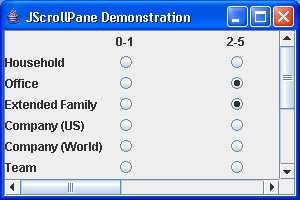
\includegraphics[scale=0.7]{imagenes/jpanels.PNG}
\caption{JScrollPane}
\end{figure}
\end{frame}

\begin{frame}
\frametitle{JScrollPane}
\begin{itemize}[<+->]
\item JSrollPane ()
\item JScrollPane(Component component)
\item JScrollPane(int ver, int hor)
\item JScrollPane(Component component, int ver, int hor)
\item  \emph{HORIZONTAL\_SCROLLBAR\_ALWAYS, HORIZONTAL\_SCROLLBAR\_AS\_NEEDED, VERTICAL\_SCROLLBAR\_ALWAYS, VERTICAL\_SCROLLBAR\_AS\_NEEDED}
\end{itemize}
\end{frame}


\subsection{JSplitPane}
\begin{frame}
\frametitle{JSplitPane}
\begin{itemize}[<+->]
\item JSplitPane()
\item JSplitPane(int)
\item JSplitPane(int, boolean)
\item JSplitPane(int, Component, Component)
\item JSplitPane(int, boolean, Component, Component)
\item donde \emph{int} puede ser \emph{HORIZONTAL\_SPLIT o VERTICAL\_SPLIT}
\item  Los parámetros \emph{Component} seleccionan los componentes izquierdo y derecho o superior e inferior, respectivamente. 
\item El parámetro \emph{boolean} El paramétodo booleano selecciona si los componentes se redibujan contínuamnete cuando el usuario arrastra el divisor.
\end{itemize}
\end{frame}

\subsection{JTabbedPane}
\begin{frame}
\frametitle{JTabbedPane}
\begin{description}[<+->]
\item[JTabbedPane()] Crea un JTabbedPane vacío, colocando las pestañas arriba.
\item[JTabbedPane(int tabPlacement)] Las pestañas se colocaran segun el valor entero: \emph{JTabbedPane.TOP, JTabbedPane.BOTTOM, JTabbedPane.LEFT, or JTabbedPane.RIGHT.}
\item[public JTabbedPane(int tabPlacement, int tabLayoutPolicy)] donde el segundo int puede ser: \emph{JTabbedPane.WRAP\_TAB\_LAYOUT o JTabbedPane.SCROLL\_TAB\_LAYOUT.}
\end{description}
\end{frame}

\begin{frame}
\frametitle{Componentes}
\framesubtitle{Componentes para introducir datos}
\begin{figure}
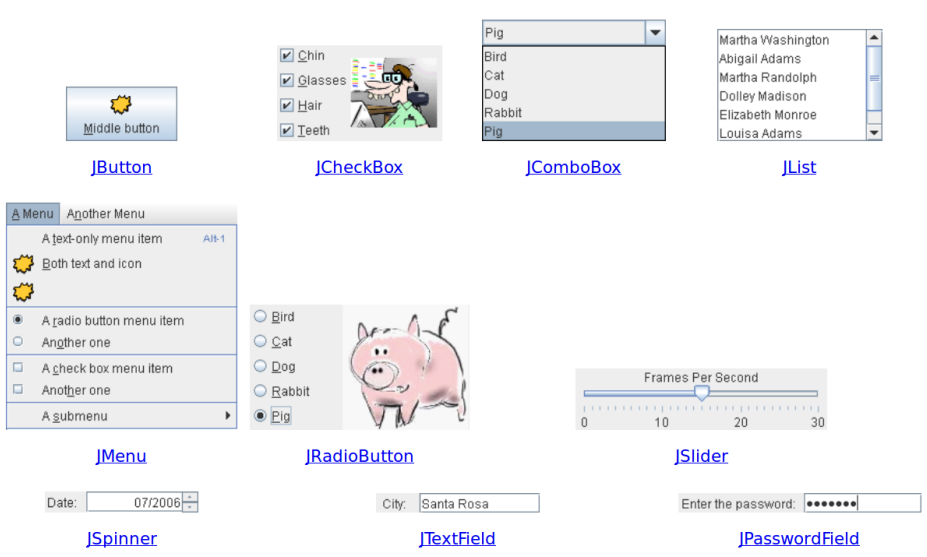
\includegraphics[width=\textwidth]{imagenes/componentes1.png}
\caption{Componentes Java GUI}
\end{figure}
\end{frame}

\begin{frame}
\frametitle{Componentes}
\framesubtitle{Componentes interactivos}
\begin{figure}
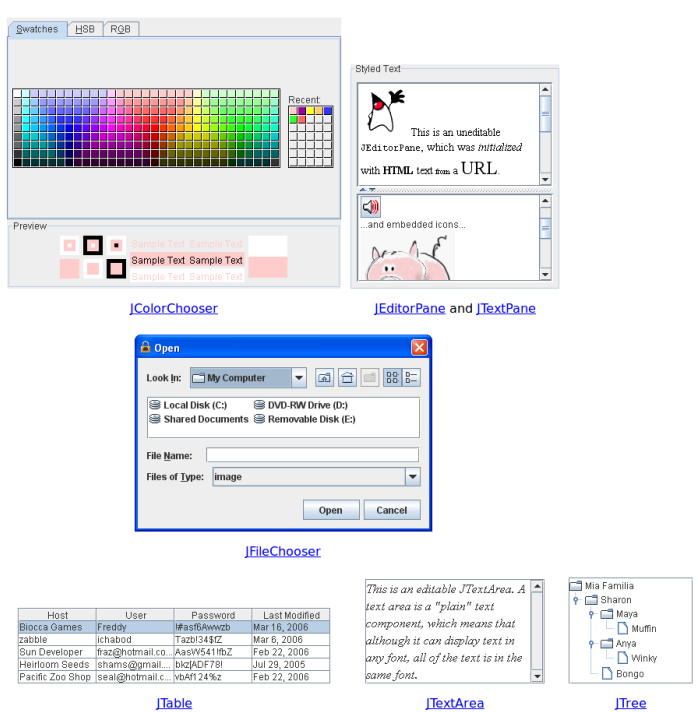
\includegraphics[scale=0.35]{imagenes/componentes2.png}
\caption{Componentes Java GUI}
\end{figure}
\end{frame}

\begin{frame}
\frametitle{Componentes}
\framesubtitle{Componentes no editables}
\begin{figure}
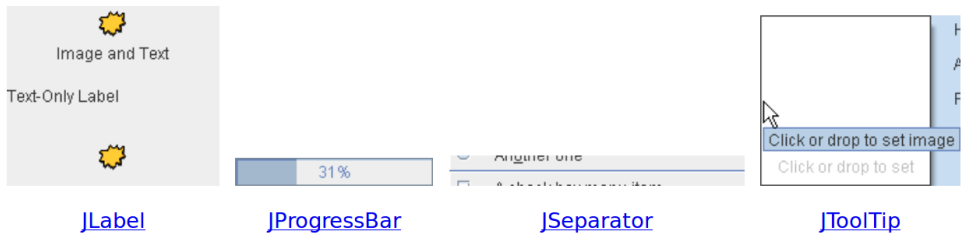
\includegraphics[width=\textwidth]{imagenes/componentes3.png}
\caption{Componentes Java GUI}
\end{figure}
\end{frame}

\section{Botones}
\begin{frame}
\frametitle{Botones}
%\begin{multicols}{2}
\begin{itemize}[<+->]
\item Botontes normales.
\item Toggle button.
\item Check button.
\item Radio button.
\end{itemize}
\pause
\begin{figure}
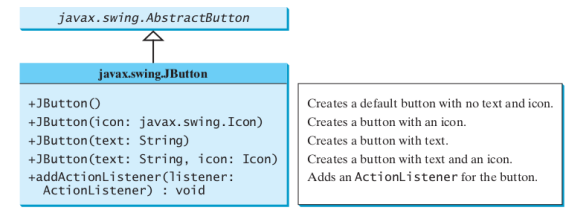
\includegraphics[scale=0.6]{imagenes/botones.png}
\end{figure}
%\end{multicols}
\end{frame}


\begin{frame}[fragile]
\frametitle{UML javax.swing.AbstractButton}
\begin{figure}
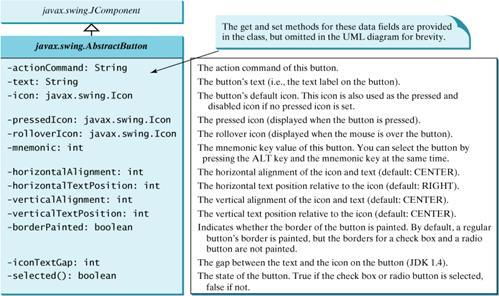
\includegraphics[width=\textwidth]{imagenes/botones.jpg}
\end{figure}
\end{frame}

\subsection{botones sencillos}
\begin{frame}[fragile]
\frametitle{Ejemplo botones}
\begin{scriptsize}
\begin{verbatim}
import javax.swing.*;
public class Botones extends JFrame
{
  public static void main (String[]args)
  {
    JFrame frame = new Botones ();
      frame.setTitle ("Botones");
      frame.setSize (200, 100);
      frame.setLocationRelativeTo (null);// Center the frame
      frame.setDefaultCloseOperation (JFrame.EXIT_ON_CLOSE);
      frame.setVisible (true);
  }
  public Botones ()
  {
    ImageIcon esIcon = new ImageIcon ("imagenes/espana.png");
    ImageIcon cuIcon = new ImageIcon ("imagenes/cuba.png");
    ImageIcon alIcon = new ImageIcon ("imagenes/alemania.png");
    JButton jbt = new JButton ("Click", esIcon);
    jbt.setPressedIcon (cuIcon);
    jbt.setRolloverIcon (alIcon);
    add (jbt);
  }
}
\end{verbatim}
\end{scriptsize}
\end{frame}

\begin{frame}
\frametitle{Alineación}
\framesubtitle{Especifica la alineación de texto e icono}
\begin{block}{Alineacion horizontal}
Se establece con \alert{setHorizontalAlignment(int)} donde int puede ser:
\begin{description}[<+->]
\item[LEADING/LEFT] izquierda
\item[RIGHT/TRAILING] derecha
\item[CENTER] centrado
\end{description}
\end{block}
\pause
\begin{block}{Alineacion vertical}
Se establece con \alert{setVerticalAlignment(int)} donde int puede ser:
\begin{description}[<+->]
\item[TOP] arriba
\item[BOTTOM] abajo
\item[CENTER] centrado
\end{description}
\end{block}
\pause
Para el texto se hace algo parecido, pero se usa \emph{setHorizontalTextPosition(int) y setVerticalTextPosition(int)}
\end{frame}

\begin{frame}
\frametitle{Alineación icono y texto} 
\begin{figure}
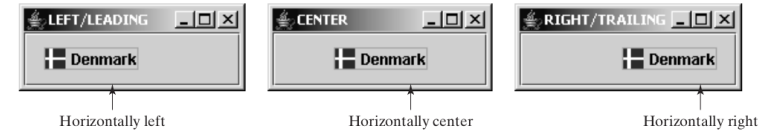
\includegraphics[scale=0.4]{imagenes/ih.png} 
\end{figure} 
\begin{figure}
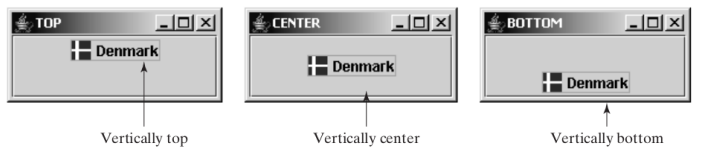
\includegraphics[scale=0.4]{imagenes/iv.png} 
\end{figure} 
\begin{figure}
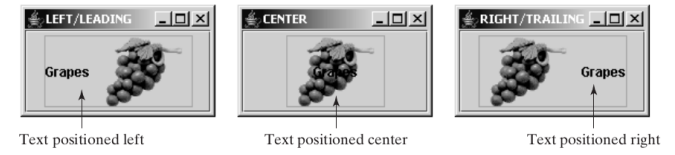
\includegraphics[scale=0.4]{imagenes/th.png} 
\end{figure} 
\begin{figure}
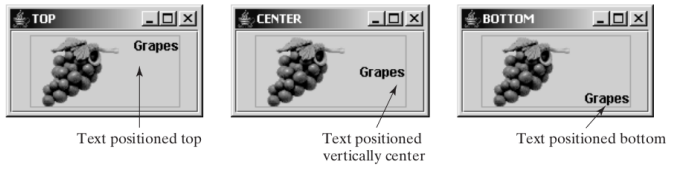
\includegraphics[scale=0.4]{imagenes/tv.png} 
\end{figure} 
\end{frame}

\subsection{toggle button}
\begin{frame}
\frametitle{toggle button}
\begin{itemize}[<+->]
\item Es un botón con dos estados.
\item La clase \alert{JToggleButton} hereda AbstractButton e implementa un \emph{toggle button}
\item Se suelen usar las clases \emph{JCheckBox y JRadioButton} para esto.
\end{itemize}
\begin{figure}
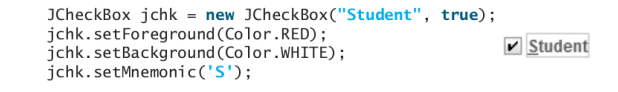
\includegraphics[scale=0.7]{imagenes/toogle1.png}
\end{figure}
\end{frame}

\subsubsection{check button}
\begin{frame}
\frametitle{check button}
\begin{figure}
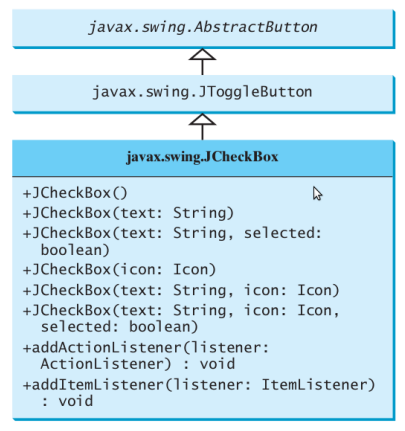
\includegraphics[scale=0.6]{imagenes/toogle.png}
\caption{UML javax.swing.JCheckBox}
\end{figure}
\end{frame}

%\begin{frame}[fragile]
%\frametitle{Eventos de check button}
%\begin{itemize}[<+->]
%\item Cuando se selecciona o deselecciona un check box este lanza un \alert{ItemEvent} y entonces un \alert{ActionEvent}
%\item Se puede procesar el \emph{ActionEvent} o el \emph{ItemEvent}
%\item Para \emph{ItemEvent} se debe implementar el método \alert{ItemListener}.
%\item Para saber si un chec box está selecionado, podemos usar el método \alert{isSelected()}
%\end{itemize}
%\pause
%\begin{verbatim}
%//para escuchar el ItemEvent
%boton.addItemListener(new ItemListener() {
%/** Manejador del ItemEvent */
%   public void itemStateChanged(ItemEvent e) {
%   ...............;
%}
%});
%\end{verbatim}
%\end{frame}

\subsubsection{radio button}
\begin{frame}[fragile]
\frametitle{radio button}
\begin{itemize}[<+->]
\item Son botones de opción de un item, dentro de un conjunto de éstos.
\item A diferencia de los check button, los \alert{radio button} NO son cuadrados, SON círculos.
\item Los \alert{Listener} son tratados de la misma manera que en los \emph{check button} 
\end{itemize}
\pause
\begin{figure}
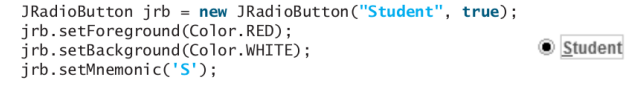
\includegraphics[scale=0.6]{imagenes/radio1.png}
\end{figure}
\end{frame}

\begin{frame}
\frametitle{check button}
\begin{figure}
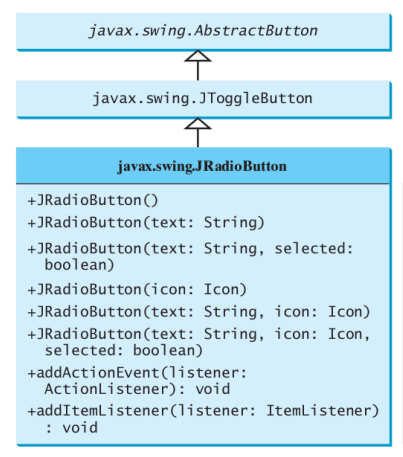
\includegraphics[scale=0.6]{imagenes/radio.png}
\caption{UML javax.swing.JRadioButton}
\end{figure}
\end{frame}

\begin{frame}[fragile]
\frametitle{gruo radio button}
\begin{itemize}[<+->]
\item Los radio button se pueden agrupar.
\item Necesitamos crear una instancia de \alert{java.swing.ButtonGroup}
\end{itemize}
\pause
\begin{verbatim}
ButtonGroup group = new ButtonGroup();
group.add(jrb1);
group.add(jrb2);
\end{verbatim}
\begin{itemize}[<+->]
\item Al agruparase \emph{jrb1} y \emph{jrb2} son mutuamente exclusivos, es decir se selección uno u otro, pero NO los dos a la vez.
\item Si no se agrupan, serían independientes y se pueden seleccionar independientemente.
\end{itemize}
\end{frame}

\section{Labels}
\begin{frame}
\frametitle{Etiquetas}
\begin{itemize}[<+->]
\item Sirven para desplegar un pequeño texto o una imagen, o ambas.
\item Suelen acompañarse con otros componentes como los \emph{textinput}
\item \alert{JLabel} hereda de \alert{JComponent} muchas propiedades útiles, similares a las de los \emph{buttons}
\begin{enumerate}
\item text
\text icon
\text horizontalAlignment
\item verticalAlignment,
\item horizontalTextPosition
\item verticalTextPosition
\item iconTextGap.
\end{enumerate}
\end{itemize}
\end{frame}


\begin{frame}
\frametitle{javax.swing.JLabel} 
\begin{figure}
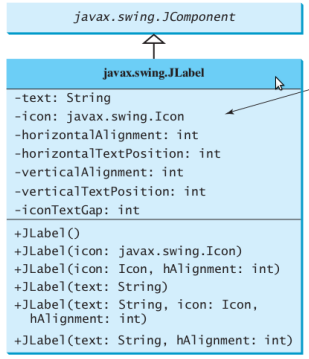
\includegraphics[scale=0.7]{imagenes/label.png} 
\end{figure} 
\end{frame}

\begin{frame}[fragile]
\frametitle{Ejemplo label}
\begin{verbatim}
// Crear una icono desde un fichero
ImageIcon icon = new ImageIcon("image/grapes.gif");
// Crea una etiqueta con texto y un icono
// con alineación horizontal y centereda
JLabel jlbl = new JLabel("Etqiueta", icon, SwingConstants.CENTER);
// Establecemos alineación del texto y separación 
//entre texto e icono
jlbl.setHorizontalTextPosition(SwingConstants.CENTER);
jlbl.setVerticalTextPosition(SwingConstants.BOTTOM);
jlbl.setIconTextGap(5);
\end{verbatim}
\end{frame}

\section{Text Fields}
\begin{frame}[fragile]
\frametitle{Campos de texto}
\begin{itemize}[<+->]
\item Sirven para desplegar texto o introducir texto (Lo mas normal).
\item \alert{JTextField} hereda de \alert{JTextComponent} el cual a su vez hereda de \alert{JComponent}
\item Se puede usar \alert{JPasswordField} donde el texto introducido es reemplazado por \emph{echo *}.
\item Puede cambiarse el caracter del echo con el método \alert{setEchoChar(char)}
\item Ejemplo:
\end{itemize}
\pause
\begin{verbatim}
JTextField mensaje = new JTextField("Entrada");
mensaje.setForeground(Color.RED);
mensaje.setHorizontalAlignment(SwingConstants.RIGHT);
\end{verbatim}
\end{frame}

\begin{frame}
\frametitle{javax.swing.JTextField} 
\begin{figure}
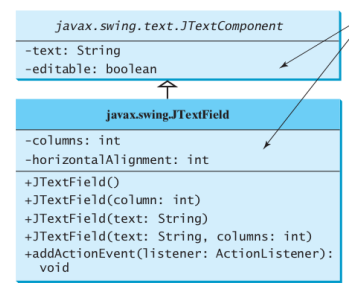
\includegraphics[scale=0.7]{imagenes/text.png} 
\end{figure} 
\end{frame}

\begin{frame}[fragile]
\frametitle{Ejemplo}
\begin{tiny}
\begin{verbatim}
import java.awt.*;
import java.awt.event.*;
import javax.swing.*;
public class TextFieldDemo extends JFrame{
  private JTextField jtfMessage = new JTextField (10);
  public static void main (String[]args)  {
    TextFieldDemo frame = new TextFieldDemo ();
      frame.pack ();
      frame.setTitle ("TextFieldDemo");
      frame.setLocationRelativeTo (null);	// Center the frame
      frame.setDefaultCloseOperation (JFrame.EXIT_ON_CLOSE);
      frame.setVisible (true);
  }
  public TextFieldDemo () {
// Crea a nuevo panel para poner label y text field
    JPanel jpTextField = new JPanel ();
    jpTextField.setLayout (new BorderLayout (5, 0));
    jpTextField.add (new JLabel ("Introduce un nuevo mensaje"),
		     BorderLayout.WEST);
    jpTextField.add (jtfMessage, BorderLayout.CENTER);
    add (jpTextField, BorderLayout.NORTH);
    jtfMessage.setHorizontalAlignment (JTextField.RIGHT);
// Register listener
    jtfMessage.addActionListener (new ActionListener () {
/** Handle ActionEvent */
	  public void actionPerformed (ActionEvent e) {
      	  JOptionPane.showMessageDialog (null,
						 jtfMessage. getText ());
				  jtfMessage.requestFocusInWindow ();}
				  });
  }
}
\end{verbatim}
\end{tiny}
\end{frame}

\section{Text Area}
\begin{frame}[fragile]
\frametitle{Area de texto}
\begin{footnotesize}
\begin{itemize}[<+->]
\item Sirven para desplegar texto en múltiles líneas.
\item Se puede crear una instanacia de \alert{JTextField}.
\item O mejor usar \alert{JTextArea} el cual a su vez hereda de \alert{JComponent}
\item Cómo \emph{JTextField}, \emph{JTextArea} hereda de \emph{JTextComponent}, el cuál contiene métodos como \alert{getText, setText, isEditable, y setEditable.}
\item Ejemplo de creación de texto con 5 filas y 20 columnas, line-wrapped, color rojo y como fuente \emph{bold, 20 pixels.}
\end{itemize}
\pause
\begin{verbatim}
JTextArea jtaNote = new JTextArea("Esto es un area de texto", 5, 20);
jtaNote.setLineWrap(true);
jtaNote.setWrapStyleWord(true);
jtaNote.setForeground(Color.red);
jtaNote.setFont(new Font("Courier", Font.BOLD, 20));
\end{verbatim}
\pause 
Podemos añadir con \alert{JScrollPane } una barra de desplazamiento:
\begin{verbatim}
JScrollPane scrollPane = new JScrollPane(jta = new JTextArea());
add(scrollPane, BorderLayout.CENTER);
\end{verbatim}
\end{footnotesize}
\end{frame}

\begin{frame}
\frametitle{javax.swing.JTextArea} 
\begin{figure}
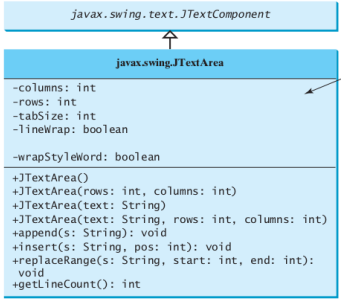
\includegraphics[scale=0.7]{imagenes/area.png} 
\end{figure} 
\end{frame}

\section{combo box}
\begin{frame}[fragile]
\frametitle{Lista de elección}
Contiene una lista de items, que el usuario puede elegir.
\begin{verbatim}
JComboBox jcb = new JComboBox(new Object[]
{"Item 1", "Item 2", "Item 3", "Item 4"});
jcb.setForeground(Color.red);
jcb.setBackground(Color.white);
jcb.setSelectedItem("Item 2");
\end{verbatim}
\begin{figure}
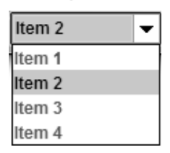
\includegraphics[scale=0.7]{imagenes/combobox.png} 
\end{figure} 
\end{frame}

\begin{frame}
\frametitle{javax.swing.JComboBox} 
\begin{figure}
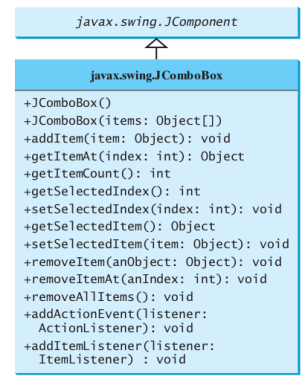
\includegraphics[scale=0.8]{imagenes/jcombobox.png} 
\end{figure} 
\end{frame}

\section{list}
\begin{frame}[fragile]
\frametitle{Lista de elección}
Similar a \emph{combo box} pero permite seleccion multiple.
\begin{verbatim}
JList jlst = new JList(new Object[]
{"Item 1", "Item 2", "Item 3", "Item 4", "Item 5",
 "Item 6"});
jlst.setForeground(Color.RED);
jlst.setBackground(Color.WHITE);
jlst.setSelectionForeground(Color.PINK);
jlst.setSelectionBackground(Color.BLACK);
jlst.setVisibleRowCount(4);
\end{verbatim}
\begin{figure}
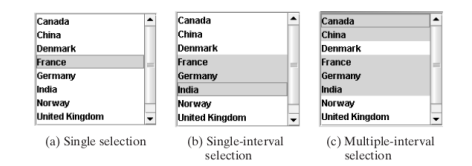
\includegraphics[scale=0.7]{imagenes/list1.png} 
\end{figure} 
\end{frame}

\begin{frame}
\frametitle{javax.swing.JComponent} 
\begin{figure}
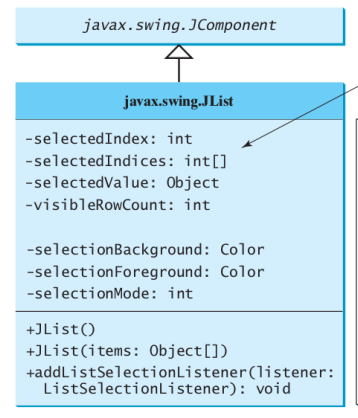
\includegraphics[scale=0.5]{imagenes/list2.png} 
\end{figure} 
\emph{selectionMode} puede ser:\\ \emph{SINGLE\_SELECTION, SINGLE\_INTERVA\_SELECTION, MULTIPLE\_INTERVAL\_SELECTION)}
\end{frame}



\section{Scroll Bars}
\begin{frame}[fragile]
\frametitle{Barrras de deslizamiento}
\begin{figure}
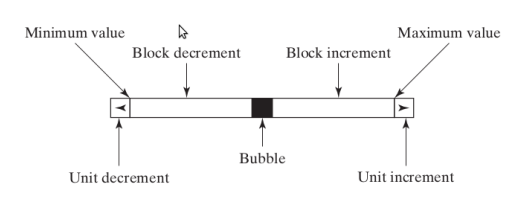
\includegraphics[scale=0.7]{imagenes/scroll1.png} 
\end{figure} 
\begin{figure}
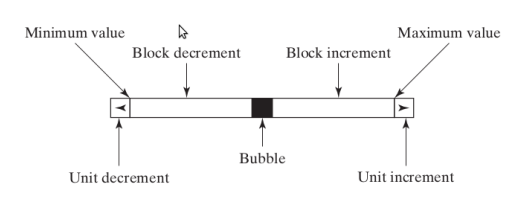
\includegraphics[scale=0.7]{imagenes/scroll1.png} 
\end{figure}
\end{frame}

\begin{frame}[fragile]
\frametitle{javax.swing.JScrollBar}
\begin{figure}
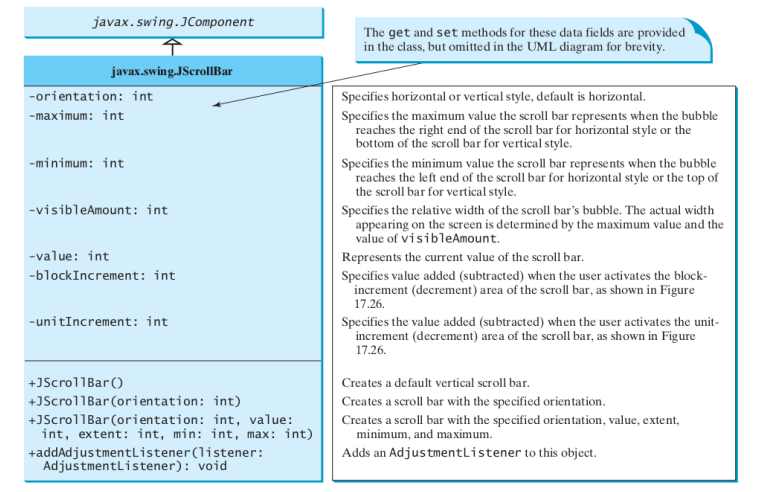
\includegraphics[scale=0.55]{imagenes/scroll2.png} 
\end{figure} 
\end{frame}


\begin{frame}
\frametitle{¿Dudas?} 
\begin{figure}

\includegraphics[scale=0.9]{imagenes/dudas.png} 
\end{figure} 
\end{frame}

\end{document}

